% Options for packages loaded elsewhere
\PassOptionsToPackage{unicode}{hyperref}
\PassOptionsToPackage{hyphens}{url}
\PassOptionsToPackage{dvipsnames,svgnames,x11names}{xcolor}
%
\documentclass[
]{article}
\usepackage{amsmath,amssymb}
\usepackage{iftex}
\ifPDFTeX
  \usepackage[T1]{fontenc}
  \usepackage[utf8]{inputenc}
  \usepackage{textcomp} % provide euro and other symbols
\else % if luatex or xetex
  \usepackage{unicode-math} % this also loads fontspec
  \defaultfontfeatures{Scale=MatchLowercase}
  \defaultfontfeatures[\rmfamily]{Ligatures=TeX,Scale=1}
\fi
\usepackage{lmodern}
\ifPDFTeX\else
  % xetex/luatex font selection
\fi
% Use upquote if available, for straight quotes in verbatim environments
\IfFileExists{upquote.sty}{\usepackage{upquote}}{}
\IfFileExists{microtype.sty}{% use microtype if available
  \usepackage[]{microtype}
  \UseMicrotypeSet[protrusion]{basicmath} % disable protrusion for tt fonts
}{}
\makeatletter
\@ifundefined{KOMAClassName}{% if non-KOMA class
  \IfFileExists{parskip.sty}{%
    \usepackage{parskip}
  }{% else
    \setlength{\parindent}{0pt}
    \setlength{\parskip}{6pt plus 2pt minus 1pt}}
}{% if KOMA class
  \KOMAoptions{parskip=half}}
\makeatother
\usepackage{xcolor}
\usepackage[margin=1in]{geometry}
\usepackage{graphicx}
\makeatletter
\def\maxwidth{\ifdim\Gin@nat@width>\linewidth\linewidth\else\Gin@nat@width\fi}
\def\maxheight{\ifdim\Gin@nat@height>\textheight\textheight\else\Gin@nat@height\fi}
\makeatother
% Scale images if necessary, so that they will not overflow the page
% margins by default, and it is still possible to overwrite the defaults
% using explicit options in \includegraphics[width, height, ...]{}
\setkeys{Gin}{width=\maxwidth,height=\maxheight,keepaspectratio}
% Set default figure placement to htbp
\makeatletter
\def\fps@figure{htbp}
\makeatother
\setlength{\emergencystretch}{3em} % prevent overfull lines
\providecommand{\tightlist}{%
  \setlength{\itemsep}{0pt}\setlength{\parskip}{0pt}}
\setcounter{secnumdepth}{-\maxdimen} % remove section numbering
%\usepackage{background}

%\backgroundsetup{
%scale=1,
%color=black,
%opacity=0.2,
%angle=0,
%pages=all,
%contents={%
%	
\includegraphics[width=\paperwidth,height=\paperheight]{img/logo_transparent.png}
%	}
%}

\usepackage{lipsum}
\usepackage{graphicx}
\usepackage{fancyhdr}
\pagestyle{fancy}
\usepackage{geometry}
\usepackage{eso-pic}
\usepackage{cuted}
\usepackage{multicol}
\usepackage{wrapfig}
\usepackage[defaultfam,tabular,lining]{montserrat} %% Option 'defaultfam'
%% only if the base font of the document is to be sans serif
\usepackage[T1]{fontenc}
\renewcommand*\oldstylenums[1]{{\fontfamily{Montserrat-TOsF}\selectfont #1}}
\usepackage[fontsize=12]{scrextend}
\fancyhf{}
%\setlength\voffset{-29pt}
%\geometry{hmargin=0pt}
\newcommand\BackgroundPic{%
\put(0,0){%
\parbox[b][\paperheight]{\paperwidth}{%
\vfill
\centering

\includegraphics[width=\paperwidth,height=\paperheight,%
keepaspectratio]{img/logo_for_background.png}%
\vfill
}}}
\setlength{\columnsep}{1cm}
\renewcommand{\headrulewidth}{0pt}
\renewcommand{\footrulewidth}{0pt}
\setlength\headheight{84.0pt}
\addtolength{\textheight}{-84.0pt}
\chead{
\includegraphics[width=\textwidth]{img/logo_banner_cropped.png}}
\pagenumbering{gobble}
\fancyhead[R]{}

% columns.tex
\newenvironment{cols}[1][]{}{}

\newenvironment{col}[1]{\begin{minipage}{#1}\ignorespaces}{%
\end{minipage}
\ifhmode\unskip\fi
\aftergroup\usignorespacesandallpars}

\def\useignorespacesandallpars#1\ignorespaces\fi{%
#1\fi\ignorespacesandallpars}

\makeatletter
\def\ignorespacesandallpars{%
	\@ifnextchar\par
		{\expandafter\ingorespacesandallpars\@gobble}%
		{}%
}
\makeatother
\ifLuaTeX
  \usepackage{selnolig}  % disable illegal ligatures
\fi
\IfFileExists{bookmark.sty}{\usepackage{bookmark}}{\usepackage{hyperref}}
\IfFileExists{xurl.sty}{\usepackage{xurl}}{} % add URL line breaks if available
\urlstyle{same}
\hypersetup{
  colorlinks=true,
  linkcolor={Maroon},
  filecolor={Maroon},
  citecolor={Blue},
  urlcolor={Blue},
  pdfcreator={LaTeX via pandoc}}

\author{}
\date{\vspace{-2.5em}2023-05-26}

\begin{document}

%\AddToShipoutPicture*{\BackgroundPic}

\vspace{2cm}

\section{Welcome to Your Microbiome!}

\begin{centering}


\begin{center}\includegraphics{Example_files/figure-latex/WdCldLrgDisplay-1} \end{center}
\end{centering}

Welcome to your IMAGINE microbiome report! In this report, you will find
an introduction to the human fecal microbiome, a description of your
personal microbiome, and some more detailed information about the
specific bacteria that were abundant in your sample.

\pagenumbering{arabic}

\newpage

\section{Introduction}

The human gut is home to hundreds of species of microbes, mostly
bacteria. In fact, your gut contains as many bacterial cells as there
are human cells in your whole body! This microbial community is known as
your `gut microbiome'.

The gut microbiome has several very important roles to play in keeping
us healthy. It helps us to break down and digest the food that we eat,
produces vitamins that we require, trains and maintains our immune
system, and serves as the first line of defense against infection from
bacteria that could do us harm.

We are still very much at the beginning of understanding all the things
the gut microbiome does, how our actions and environment affect it, and
how we can use it to keep people healthier and living longer. The
\textbf{\color{Cerulean}MAGIC} study (a sub-study of the
\textbf{\color{RedOrange}IMAGINE} study that you are participating in)
is an ambitious project that will improve our understanding of how three
important variables (genes, diet, and mental health) impact the gut
microbiome in people with inflammatory bowel

\begin{wrapfigure}{r}{0.18\textwidth}
\begin{center}
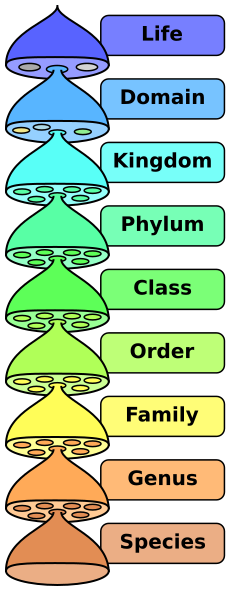
\includegraphics[width=0.18\textwidth]{img/Biological_classification_L_Pengo_vflip.png}
\end{center}
\end{wrapfigure}

disease (IBD) and irritable bowel syndrome (IBS), and in turn how all
four factors together impact the disease course.

\subsection{Studying the microbiome}

A key component of the MAGIC study is generating microbiome profiles for
each participant in the study. So, how do we do that?

Bacteria, just like plants and animals, can be grouped together into
closely related groups called \textbf{species}. Those species can then
be grouped together into bigger groups called \textbf{genera} (singular:
genus), and genera can be grouped together into \textbf{families}, and
so on up the tree of life.

Each bacterial species has a unique genetic ``barcode'' that can be used
to identify it. To determine the composition of each sample's
microbiome, we extract the DNA from your stool sample and then isolate
and sequence these bacterial DNA barcodes. We don't sequence any human
DNA, just the bacterial barcodes. We generate 10,000 to 50,000 barcode
sequences per sample. Each sequence is then labeled with its taxonomic
identity (which species, genus, family, etc. it belongs to) and the
number of bacteria present in each species is counted.

You can think of the bacteria in your gut like a jar of jelly beans. The
barcode tells us what colour each jelly bean is, and the number of times
we see that barcode in our sequences tells us how many jelly beans there
are of that colour. This allows us to sort the bacteria into species and
generate the ``taxonomic bar chart'' you'll see in this document.

JELLY BEAN IMAGE

As there are hundreds of species in a sample, we quickly run out of
colours! Therefore, we will use the categories at the genus or family
level, and also only display the bacteria that are abundant enough to
show up clearly on the chart.

These microbiome profiles are only the beginning. We use the information
in them to compare profiles between healthy controls and people with
IBD/IBS, and to investigate ways that a person's microbiome changes with
their health status. We also try to identify individual microbes that
might be associated with specific illnesses. Understanding these
associations between our microbes and our health will lead to new
treatments that target the microbiome directly: increasing ``good''
bacteria and decreasing ``bad'' bacteria.

\newpage

\vspace*{\fill}

\begin{multicols}{2}
[\textbf{Your Sample}]

\begin{small}
This bar chart shows your personal fecal bacterial community. 
Bacteria are grouped into \textbf{families} based on how closely related
they are.

The bar chart is stacked from most abundant bacterial family on the 
bottom, to least abundant on the top, with very low-abundance 
bacteria grouped together as "Other". Next to it is a chart showing
the average community of all the people who participated in the study,
and across the bottom are four anonymous individuals chosen to show
the range of variation in this study. As you can see, it's quite wide!
\end{small}
\columnbreak

\includegraphics{Example_files/figure-latex/BarPlotDisplay-1.pdf}

\end{multicols}

\begin{center}\includegraphics{Example_files/figure-latex/unnamed-chunk-5-1} \end{center}
\vspace*{\fill}
\newpage

\begin{multicols}{2}
\raggedcolumns

\begin{center}\includegraphics{Example_files/figure-latex/WdCldSmlDisplay-1} \end{center}

\columnbreak

\vspace*{1cm}
\section{$\boldsymbol{\leftarrow}$ More Detail}
\begin{small}
This word cloud shows your personal bacterial community at a finer 
level of detail. Within each family, bacteria can be subdivided into 
several \textbf{genera} (singular, \textbf{genus}). The size of each word
represents the relative abundance of that genus, and the colour shows
which family that genus comes from.
\end{small}
\vspace*{\fill}

\end{multicols}

\begin{multicols}{2}
\raggedcolumns

\vspace*{\fill}
\section{You Are Here $\boldsymbol{\rightarrow}$}
\begin{small}
There are over 1,000 people participating in this study so far! We have 
graphed everyone together based on how similar or different their gut
microbiomes were. In the next graph, points that are closer together
are more similar to each other, and points that are farther apart are
more different. Your sample is shown in green. Remember that your 
position in this graph doesn't say anything about how healthy your
gut microbiome is. As we've seen above, there is a wide range of 
normal variation in the human gut.
\end{small}

\vspace*{\fill}
\columnbreak

\vspace*{1cm}

\begin{center}\includegraphics{Example_files/figure-latex/BrayPlotDisplay-1} \end{center}

\vspace*{\fill}

\end{multicols}

\newpage

\section{Your Bacterial Families}

Everyone's microbiome is different. In your microbiome, the four most
abundant bacterial families were \textit{Lachnospiraceae},
\textit{Ruminococcaceae}, \textit{Bacteroidaceae}, and
\textit{Oscillospiraceae*}. Here is a little bit of information about
what functions these four familes perform in the gut.

\subsection{Lachnospiraceae}

\begin{small}
This family of bacteria is found in the gut and plays an important role in the 
breakdown of complex carbohydrates. Lachnospiraceae are known for their ability 
to ferment a variety of dietary fibers, producing short-chain fatty acids 
(SCFAs) such as butyrate, propionate, and acetate. These SCFAs provide an energy
source for the body, improve gut health, and have anti-inflammatory properties. 
Research has also linked Lachnospiraceae to improved metabolic health and a 
reduced risk of obesity.
\end{small}

\subsection{Ruminococcaceae}

\begin{small}
Ruminococcaceae are involved in the fermentation of dietary fiber and the 
production of SCFAs. These bacteria also play a role in regulating the immune 
system and maintaining gut health. Research has shown that reduced levels of 
Ruminococcaceae in the gut are associated with inflammatory bowel diseases such 
as Crohn's disease and ulcerative colitis.
\end{small}

\subsection{Bacteroidaceae}

\begin{small}
Bacteroidaceae is a family of bacteria found in the gut that are involved in the
breakdown of complex carbohydrates, such as dietary fibers and resistant 
starches. These bacteria produce enzymes that can break down plant-based foods, 
making the nutrients more accessible to the body. Bacteroidaceae also play a 
role in regulating the immune system and maintaining gut health, and their 
presence has been associated with a reduced risk of inflammatory bowel diseases.
\end{small}

\subsection{Oscillospiraceae}

\begin{small}
Members of the Oscillospiraceae family of bacteria have been linked to improved 
glucose metabolism and may have a role in regulating blood sugar levels. These 
bacteria are involved in the breakdown of complex carbohydrates and the 
production of SCFAs such as butyrate, which have been shown to improve gut 
health and protect against inflammation.
\end{small}

\end{document}
